\documentclass[12pt,a4paper]{article}
\usepackage[utf8]{inputenc}
\usepackage{amsmath}
\usepackage{amsfonts}
\usepackage{amssymb}
\usepackage{makeidx}
\usepackage{graphicx}
\usepackage[left=2cm,right=2cm,top=2cm,bottom=2cm]{geometry}

\title{\textbf{Sistemas electronicos de interfaz\\EV 1.2. Octoacopladores y relevadores}
\author{Angel Eraclio Briano Garcia 18311625\\Josue Natanael Orozco Nevares 18311797}
\date{4 de octubre del 2019}}




\begin{document}
\maketitle

\begin{figure}[h!]
\centering

\includegraphics[width=10cm]{UPCDLZMDG5783-logo.png} 
\end{figure}
\newpage

\section{Objetivo}
Conocer el funcionamiento de un PLC desde construirlo hasta la programaciòn del mismo.

\section{Materiales}
-Protoboard\\-Caimanes\\-Cables para arduino\\-Arduino UNO\\-Resistencias variadas\\-Octoacopladores 4N25\\-Relevadores de 5V\\-Fuente de voltaje

\section{Procedimiento}
\subsection{Primer paso} Se comenzo por armar las dos partes de nuestro PLC, uno que estaba compuesto por la parte de los octoacopladores junto con los leds para asi poder lograr ver la señal, que es la siguiente:

\begin{figure}[h!]
\centering
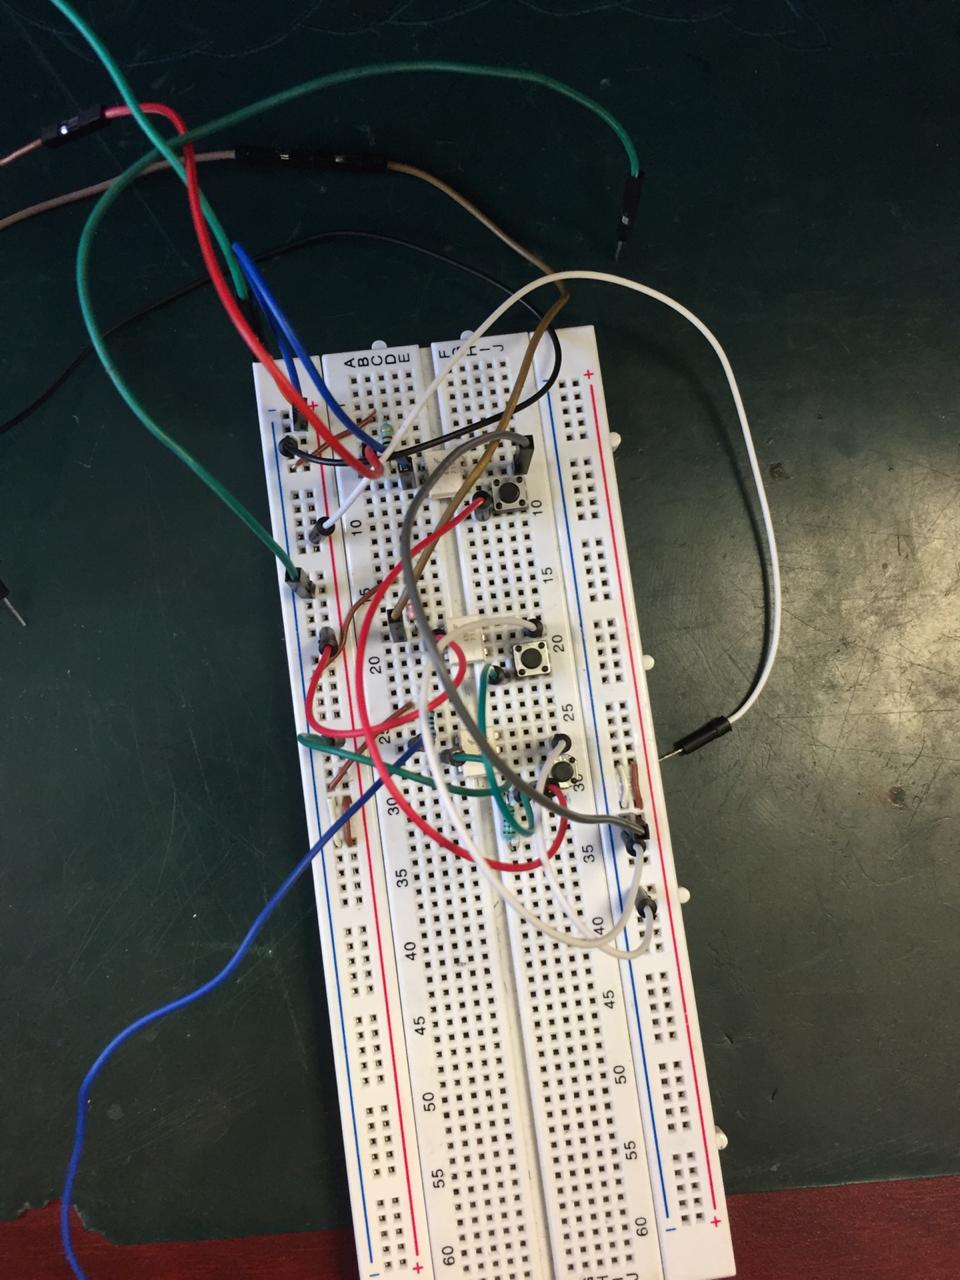
\includegraphics[width=10cm]{primeraimagen.jpeg} 
\end{figure}
\newpage

\subsection{Segundo paso} Una vez logrado el paso anterior se comprueba haciendo una conexion simple para probar el funcionamiento de los botones con los leds, en dado caso de falla verificar inmediatamente.

\subsection{Tercer paso} Cuando se tenga la parte del primer circuito se procede a realizar la parte de los relays ademas de comprobar que se disparen correctamente, el circuito terminado es el siguiente:

\begin{figure}[h!]
\centering
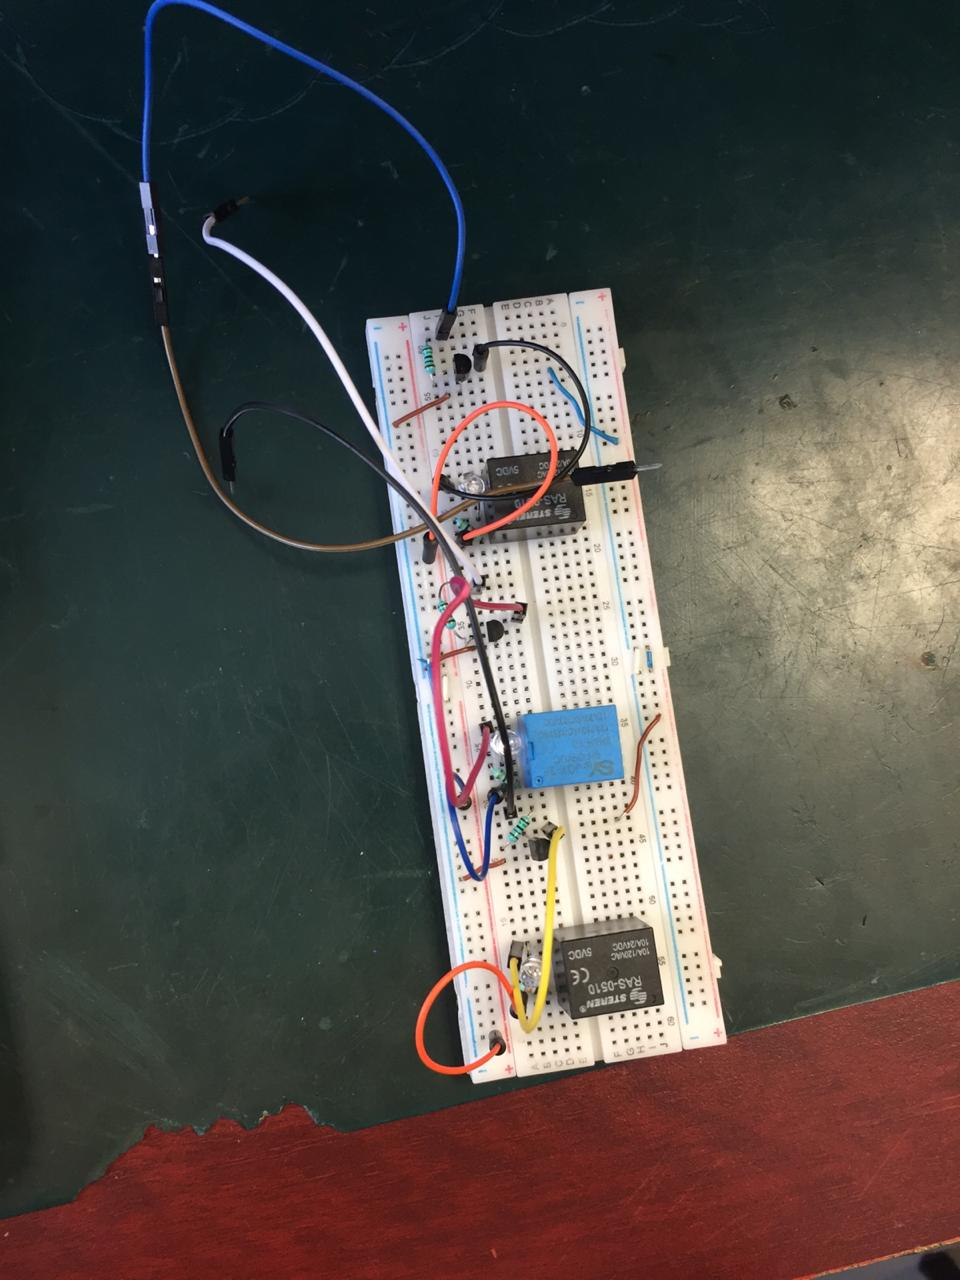
\includegraphics[width=5cm]{segundaimagen.jpeg} 
\end{figure}

\section{Cuarto paso}
Despues de lograr armar y haber comprobado ambos circuitos de que funcionan autonomamente, se procede a unirlos con el puente que en este caso sera nuestro arduino, se procedera a crear el programa para nuestro PLC, ademas de conectar adecuadamente las entradas y las salidas, recordar que son tres entradas y tres salidas como se muestra acontinuaciòn:

\begin{figure}[h!]
\centering
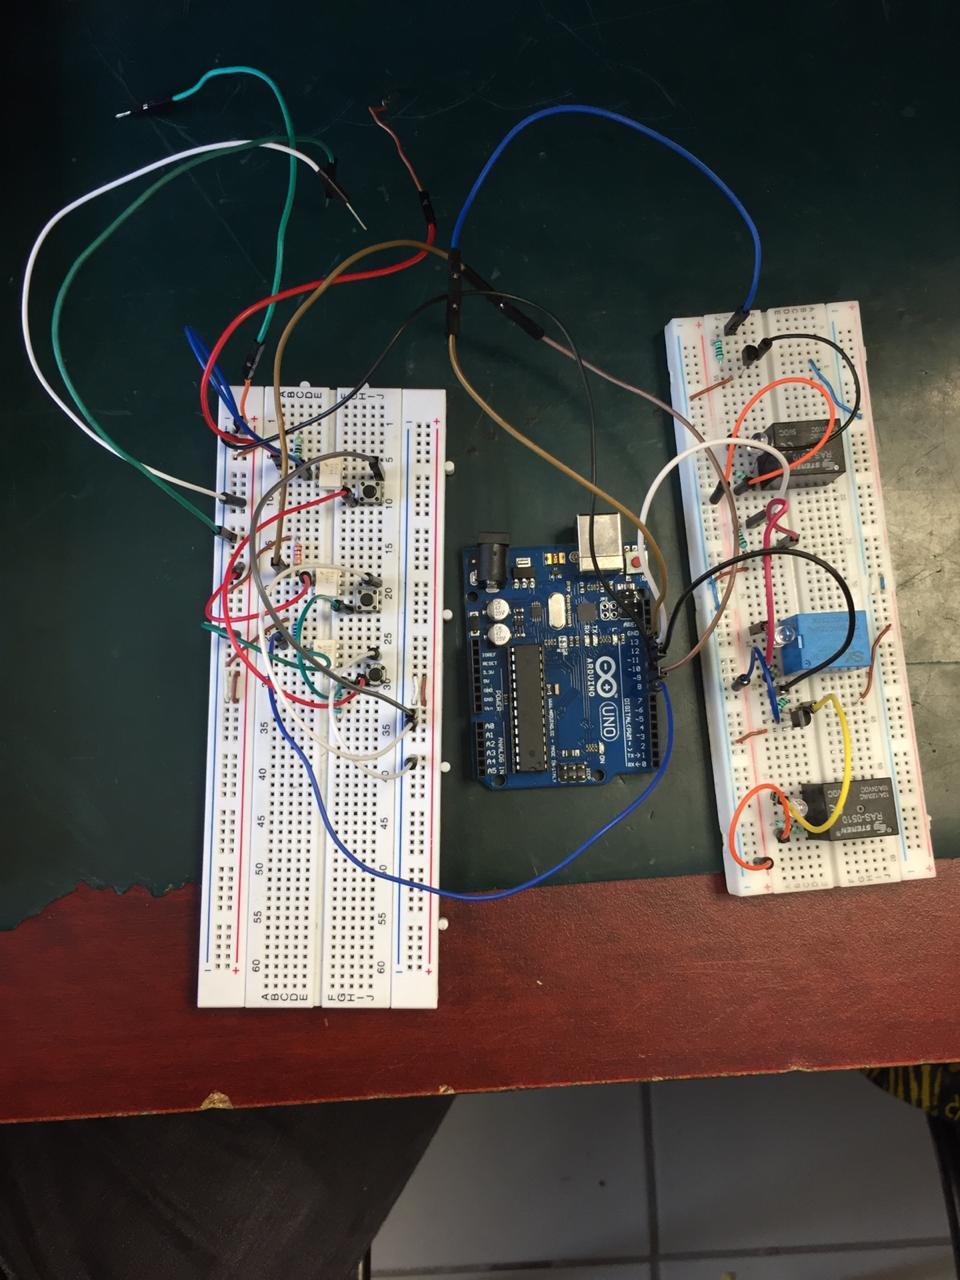
\includegraphics[width=6cm]{terceraimagen.jpeg} 
\end{figure}

\section{Resultados}
Al momento de ensamblar ambos circuitos al arduino y haber cargado el programa a la tarjeta, funciono al 85 porciento de lo que esperabamos, debido a que el segundo relay mantenia una respuesta erronea comparada con la de los otros dos relays debido a que presentaba un poco de retraso de acciòn, de algun modo mantenia un delay muy pequeño pero no era lo esperado, afortunadamente se descubrio que la falla procedia directamente de la salida del arduino ya que se comprobo cambiandolo a otro puerto y mostro su eficacia, no habia falla de conecxiòn alguna. Un caso bastante curioso.



\end{document}